Spiral Galaxies oder Tentai Show
(japanisch \begin{CJK}{UTF8}{min}天体ショー\end{CJK})
ist ein Logikrätsel, welches auf einem $n\times n$-Feld gespielt wird.
Das Feld muss nach folgenden Regeln in Gebiete unterteilt werden:
\begin{enumerate}
\item
Jedes Feld ist in genau einem der Gebiete enthalten.
\item
Jedes Gebiet enthält genau einen der grauen Punkte.
\item
Jedes Gebiet ist punktsymmetrisch bezüglich des grauen Punktes.
\end{enumerate}
Hier ein Spiral Galaxies-Rätsel (links) mit Lösung (rechts):
\begin{center}
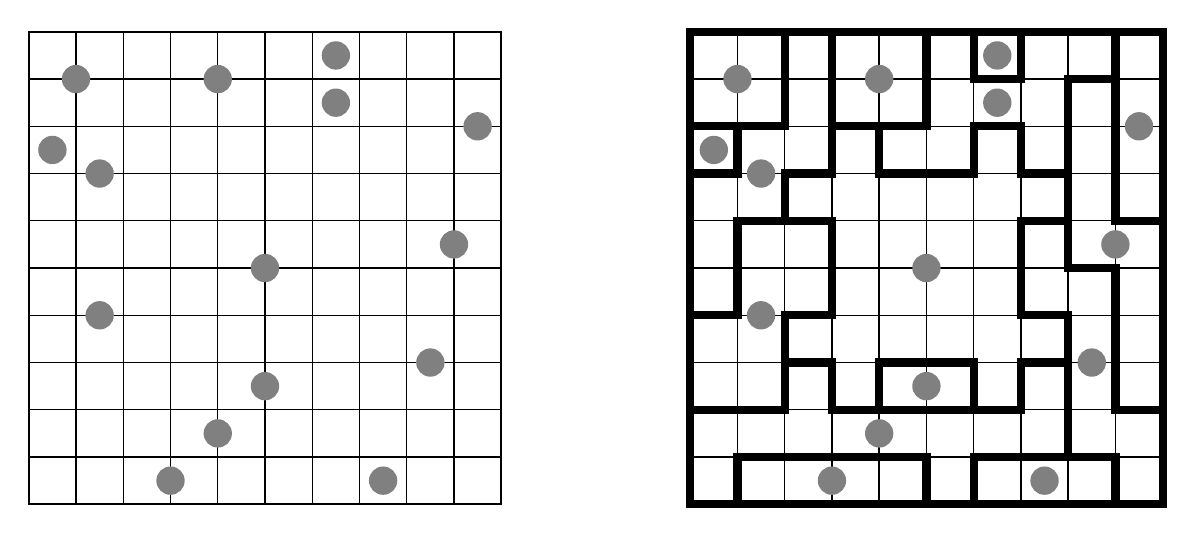
\begin{tikzpicture}[>=latex,thick,scale=0.6]

\def\spielfeld{
	\foreach \a in {1,...,9}{
		\draw[line width=0.5pt] (\a,0) -- (\a,10);
		\draw[line width=0.5pt] (0,\a) -- (10,\a);
	}
	\draw (0,0) rectangle (10,10);
}

\def\punkt#1{
	\fill[color=gray] #1 circle[radius=0.3];
}

\def\vorgaben{
	\punkt{(3,0.5)}
	\punkt{(7.5,0.5)}
	\punkt{(4,1.5)}
	\punkt{(5,2.5)}
	\punkt{(8.5,3)}
	\punkt{(1.5,4)}
	\punkt{(5,5)}
	\punkt{(9,5.5)}
	\punkt{(1.5,7)}
	\punkt{(0.5,7.5)}
	\punkt{(9.5,8)}
	\punkt{(6.5,8.5)}
	\punkt{(1,9)}
	\punkt{(4,9)}
	\punkt{(6.5,9.5)}
}

\def\loesung{
	\draw[line width=3.0pt]
		   (0,0) -- (1,0) -- (1,1) -- (5,1) -- (5,0) -- (6,0) -- (6,1)
		-- (8,1) -- (8,3) -- (7,3) -- (7,2) -- (3,2) -- (3,3) -- (2,3)
		-- (2,2) -- (0,2) -- cycle;
	\draw[line width=3.0pt]
		   (1,0) -- (5,0) -- (5,1) -- (1,1) -- cycle;
	\draw[line width=3.0pt]
		   (6,0) -- (9,0) -- (9,1) -- (6,1) -- cycle;
	\draw[line width=3.0pt]
		   (9,0) -- (10,0) -- (10,2) -- (9,2) -- (9,5) -- (8,5)
		-- (8,6) -- (7,6) -- (7,4) -- (8,4) -- (8,1) -- (9,1)
		-- cycle;
	\draw[line width=3.0pt]
		   (0,2) -- (2,2) -- (2,4) -- (3,4) -- (3,6) -- (1,6) -- (1,4)
		-- (0,4) -- cycle;
	\draw[line width=3.0pt]
		   (3,2) -- (4,2) -- (4,3) -- (6,3) -- (6,2) -- (7,2) -- (7,3)
		-- (8,3) -- (8,4) -- (7,4) -- (7,6) -- (8,6) -- (8,7) -- (7,7)
		-- (7,8) -- (6,8) -- (6,7) -- (4,7) -- (4,8) -- (3,8) -- (3,7)
		-- (2,7) -- (2,6) -- (3,6) -- (3,4) -- (2,4) -- (2,3) -- (3,3)
		-- cycle;
	\draw[line width=3.0pt]
		   (9,2) -- (10,2) -- (10,6) -- (9,6) -- (9,9) -- (8,9)
		-- (8,5) -- (9,5) -- cycle;
	\draw[line width=3.0pt]
		   (9,6) -- (10,6) -- (10,10) -- (9,10) -- cycle;
	\draw[line width=3.0pt]
		   (0,4) -- (1,4) -- (1,6) -- (2,6) -- (2,7) -- (3,7) -- (3,10)
		-- (2,10) -- (2,8) -- (1,8) -- (1,7) -- (0,7) -- cycle;
	\draw[line width=3.0pt]
		   (0,7) -- (1,7) -- (1,8) -- (0,8) -- cycle;
	\draw[line width=3.0pt]
		   (0,8) -- (2,8) -- (2,10) -- (0,10) -- cycle;
	\draw[line width=3.0pt]
		   (3,8) -- (5,8) -- (5,10) -- (3,10) -- cycle;
	\draw[line width=3.0pt]
		   (4,7) -- (6,7) -- (6,8) -- (7,8) -- (7,7) -- (8,7) -- (8,9)
		-- (9,9) -- (9,10) -- (7,10) -- (7,9) -- (6,9) -- (6,10)
		-- (5,10) -- (5,8) -- (4,8) -- cycle;
	\draw[line width=3.0pt]
		   (6,9) -- (7,9) -- (7,10) -- (6,10) -- cycle;
}

\begin{scope}[xshift=-7cm]
	\spielfeld
	\vorgaben
\end{scope}

\begin{scope}[xshift=7cm]
	\spielfeld
	\vorgaben
	\loesung
\end{scope}

\end{tikzpicture}
\end{center}
Kann eine nichtdeterministische Turing-Maschine in polynomieller Zeit 
entscheiden, ob ein Spiral Galaxies-Rätsel eine Lösung hat?

\thema{NP}
\thema{polynomieller Verifizierer}

\begin{loesung}
Das Problem ist sicher entscheidbar, indem man alle endlich vielen
möglichen Unterteilungen des Gebietes daraufhin überprüft, ob sie
die Regeln erfüllt.

Eine nichtdeterministische Turing-Maschine kann das Problem in 
polynomieller Zeit entscheiden, wenn es einen polynomiellen
Verifizierer gibt.
Ein solcher verwendet als Zertifikat eine Nummerierung der Gebiete
und für jedes Feld die Nummer des Gebietes, zu dem es gehört.
Damit sind folgende Verifikationen durchzuführen:
\begin{center}
\begin{tabular}{>{$}c<{$}|p{12cm}|>{$}c<{$}}
\text{Regel}&Verifikation&\text{Laufzeit} \\
\hline
0
&Falls ein Gebiet mehr als ein Feld hat, überprüfe, dass jedes Feld
des Gebietes einen Nachbarn in dem Gebiet hat.
&O(n^2)
\\
1
&Ist automatisch erfüllt 
&0
\\
2
&Für jeden grauen Punkt (von denen es höchstens $n^2$ gibt) überprüfe,
dass alle Felder, auf denen der Punkt liegt, zum gleichen Gebiet gehören
&O(n^2\cdot n^2)
\\
3
&Für jeden grauen Punkt und für jedes Feld im gleichen Gebiet überprüfe,
dass das punksymmetrisch gespiegelte Feld zum gleichen Gebiet gehört.
&O(n^4)
\\
\hline
&Total&O(n^4)
\end{tabular}
\end{center}
Damit ist gezeigt, dass der Verifizierer polynomielle Laufzeit hat.
Somit ist Spiral Galaxies in NP.
\end{loesung}

\begin{bewertung}
Entscheidbarkeit ({\bf E}) 1 Punkt,
Prinzip Verifizierer ({\bf V}) 1 Punkt,
Zertifikat spezifiziert ({\bf Z}) 1 Punkt,
Laufzeitschätzung ({\bf L}) 2 Punkte,
Schlussfolgerung polynomieller Verifizierer ({\bf S}) 1 Punkt.
\end{bewertung}


